\chapter{힉스 메커니즘: 게이지 보손은 어떻게 질량을 얻는가}

이제 앞선 강의에서 다룬 두 가지 생각을 결합해 보자. 전역 \(U(1)\) 대칭성이 깨진 복소 스칼라장에는 질량이 있는 방사 방향 진동과 질량이 없는 각방향 진동이 있다. 국소적으로 불변인 \(U(1)\) 이론에는 질량이 없는 게이지장이 있다. 스칼라장이 전하를 띠고 평형 크기가 영이 아니면, 이 두 진술을 단순히 더할 수는 없다. 각방향 모드와 게이지장이 결합하면 게이지장이 질량을 얻고, 겉보기의 골드스톤 보손은 독립적인 입자가 아니게 되며, 방사 방향 힉스 모드는 남는다.

광자를 모형 게이지 보손으로 삼겠지만, 물리적 결론의 대상으로 삼지는 않는다. 진공에서는 전자기 \(U(1)\)가 깨지지 않으므로 실제 광자는 질량이 없다. 게이지 군과 스칼라 다중항이 더 복잡한 전약 이론에서는 같은 메커니즘이 \(W^\pm\)와 \(Z\)에 작용한다. 아벨 모형은 군론으로 메커니즘을 가리지 않고 드러내 준다.

\begin{classroomqa}\audiencequestion{앞서 한 논의는 힉스 메커니즘이 실제 광자에 질량을 준다는 뜻이었나요?\lecturetimestamp{00:00:23}}\lecturerresponse{아닙니다. 광자와 관련된 \(U(1)\)가 깨진 상에 있다면 \emph{어떻게 될지} 묻는 것입니다. 그런 가상의 광자는 질량을 얻게 됩니다. 실제 전자기 진공은 그런 상에 있지 않습니다. 입자물리학에서 이 메커니즘은 대신 \(W\)와 \(Z\)의 질량을 설명합니다.}\end{classroomqa}

전하 보존과 관련된 대칭은 위상 회전입니다.
\begin{equation}
  \phi(x)\longmapsto e^{i\theta}\phi(x),
\end{equation}
이는 \(U(1)\)라 불리는 내부 회전이다. 초전도체는 깨진 상의 실제 유사 사례다. 초전도체 내부에서는 전자기장이 유한한 침투 깊이를 가지며, 중요한 여러 측면에서 질량이 있는 장처럼 거동한다. 초전도체 바깥에서는 익숙한 질량 없는 광자가 다시 나타난다.

\section{장에 대한 질량의 의미}

\subsection{분산 관계와 영운동량 에너지 간극}

힉스장을 도입하기 전에 질량이 정확히 무엇을 뜻하는지 정해 두는 편이 좋다. 파동에서는
\begin{equation}
  E=\hbar\omega,
  \qquad
  p=\hbar k,
  \label{eq:l08-quantum-wave}
\end{equation}
따라서 \((E,p)\) 그래프와 \((\omega,k)\) 그래프는 \(\hbar\) 계수만큼의 차이를 제외하면 같은 정보를 담는다. 빈 공간에서 질량 없는 상대론적 여기 상태는 다음을 만족한다.
\begin{equation}
  E=c|p|,
  \qquad
  \omega=c|k|.
  \label{eq:l08-massless-dispersion}
\end{equation}
\(k\)의 두 부호는 서로 반대인 전파 방향을 구분한다. 핵심은 \(\omega\)가 \(k\)와 함께 0으로 간다는 점이다.

질량이 있는 상대론적 입자는 다음 관계를 따른다.
\begin{equation}
  E^2=c^2p^2+m^2c^4.
  \label{eq:l08-massive-dispersion}
\end{equation}
단위계 \(c=\hbar=1\)에서는
\begin{equation}
  \omega^2=k^2+m^2.
\end{equation}
\(k=0\)에서 에너지는 \(E=mc^2\)이며, 자연 단위계에서는 간단히 \(m\)이다.
따라서 질량은 운동량이 영인 모드의 영이 아닌 에너지 간극이다.

\begin{figure}[htbp]
\centering
\begin{adjustbox}{max width=\linewidth}
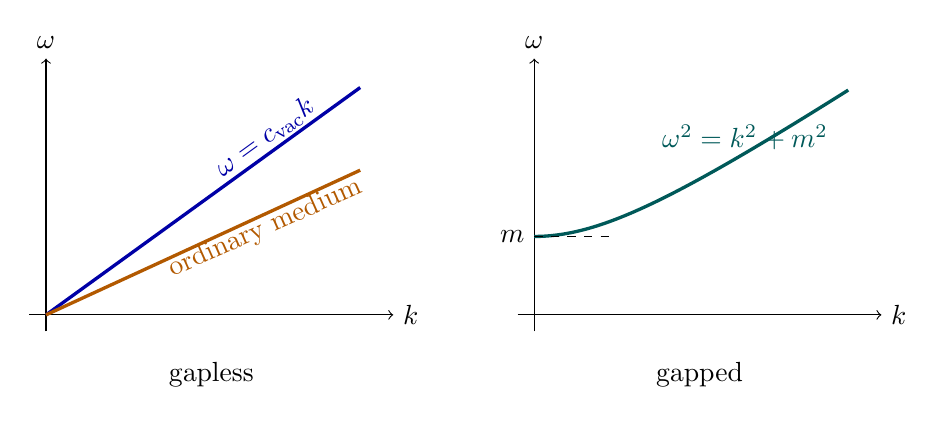
\begin{tikzpicture}[x=1.05cm,y=1.05cm]
  \begin{scope}
    \draw[->] (-0.2,0) -- (4.2,0) node[right] {\(k\)};
    \draw[->] (0,-0.2) -- (0,3.1) node[above] {\(\omega\)};
    \draw[very thick,blue!65!black] (0,0) -- (3.8,2.75);
    \draw[very thick,orange!70!black] (0,0) -- (3.8,1.75);
    \node[blue!65!black,rotate=36] at (2.65,2.15)
      {\(\omega=c_{\rm vac}k\)};
    \node[orange!70!black,rotate=24] at (2.65,1.05)
      {ordinary medium};
    \node[below] at (2,-0.45) {gapless};
  \end{scope}
  \begin{scope}[xshift=6.2cm]
    \draw[->] (-0.2,0) -- (4.2,0) node[right] {\(k\)};
    \draw[->] (0,-0.2) -- (0,3.1) node[above] {\(\omega\)};
    \draw[very thick,domain=0:3.8,samples=120,smooth,teal!70!black]
      plot (\x,{sqrt(0.9+0.45*\x*\x)});
    \draw[dashed] (0,0.95) -- (1.0,0.95);
    \node[left] at (0,0.95) {\(m\)};
    \node[teal!70!black] at (2.55,2.15)
      {\(\omega^2=k^2+m^2\)};
    \node[below] at (2,-0.45) {gapped};
  \end{scope}
\end{tikzpicture}
\end{adjustbox}
\caption{전파 속도가 달라지면 간극이 없는 분산 관계의 기울기가 달라진다. 여기에 질량을 부여하면 \(k=0\)에서 영이 아닌 간극이 생긴다.}
\label{fig:l08-dispersion}
\end{figure}

일반적인 투명 물질은 파동의 위상 속도를 낮출 수 있지만, 이 상대론적 질량 간극을 만들지는 않는다. 경계면에서는 입사파의 진동수가 고정되고 파수는 매질의 분산 관계에 맞춰 조정된다. 기울기를 바꾸는 것은 절편을 올리는 것과 같지 않다.
\editorialnote{물질에는 여러 전자기 분지가 있을 수 있으며, 플라스마나 공명 매질에는 영이 아닌 플라스마 주파수 간극이 있을 수 있다. 강의에서 비교하는 것은 일반적인 굴절 분지와 초전도 응답이다. 더 일반적으로 간극이 없다는 것은 \(\omega(k)\to0\)이며, 이 극한은 \(k\to0\)에서 취한다. 모든 비상대론적 매질에서 분산 관계가 정확히 선형일 필요는 없다.}

\begin{classroomqa}\audiencequestion{프리즘을 통과하는 경우처럼, 광자는 물질 속을 지나갈 때마다 질량을 얻나요?\lecturetimestamp{00:03:02}}\lecturerresponse{아닙니다. 굴절은 진동수와 파수의 관계를 바꾸어 전파 속도를 바꿀 수 있지만, 분산 가지는 여전히 \(k=0\)에서 \(\omega=0\)을 지난다. 반면 초전도상에서는 전자기 응답의 역침투 길이가 유한해지며, 이것이 질량의 유사량에 해당한다.}\end{classroomqa}

\begin{classroomqa}\audiencequestion{일정한 진동수의 빛이 유리에 들어가면 파수가 바뀌나요?\lecturetimestamp{00:09:20}}\lecturerresponse{그렇습니다. 정지한 경계면에서 시간 병진 대칭이 보존되므로 진동수는 고정된다. 유리에서는 분산 곡선의 기울기가 다르므로 같은 \(\omega\)에 대응하는 \(k\)가 달라지고, 따라서 파장도 달라진다.}\end{classroomqa}

기울기
\begin{equation}
  v_g=\frac{d\omega}{dk}
\end{equation}
는 파동 묶음의 군속도다. 이 기울기가 \(k\)에 따라 달라지면 푸리에 성분마다 속도가 달라져 파동 묶음이 분산한다. 그래서 \(\omega(k)\)라는 관계를 \emph{분산 관계}라고 부른다.

\begin{classroomqa}\audiencequestion{이 곡선의 이름은 무엇이며, 기울기는 무엇을 나타내나요?\lecturetimestamp{00:11:02}}\lecturerresponse{이 곡선은 분산 관계다. 곡선의 도함수 \(d\omega/dk\)는 군속도다. 기울기가 일정하면 모든 파장이 같은 속도를 가지지만, 기울기가 변하면 파동 묶음이 퍼진다. 여기서 결정적인 구분은 곡선이 원점을 지나는지, 아니면 간극이 있는지다.}\end{classroomqa}

\subsection{균일한 진동은 정지한 입자다}

모드 \(k=0\)의 파장은 무한대다. 장은 모든 곳에서 같은 크기만큼 변위한다. 균일하게 변위시킨 뒤 놓아 보자. 장이 영이 아닌 진동수로 진동한다면 이에 대응하는 양자는 영이 아닌 정지 에너지를 가지므로 질량이 있다. 그 방향으로 복원력이 없다면 진동수는 영이 되고 모드는 질량이 없다.

이 진술은 고전적인 내용이다. 공간적으로 떨어진 입자들이 양자 중첩 상태에 있어야 하는 것은 아니다. 균일한 고전 장 배치는 단지 공간 전체에 동일한 장의 값이 놓인 상태다.

\begin{classroomqa}\audiencequestion{장 전체를 함께 이동시키는 것이 양자 얽힘과 같은 것인가요?\lecturetimestamp{00:10:04}}\lecturerresponse{아닙니다. 균일한 고전 장은 하나의 고전적 배치다. 얽힘은 위--아래와 아래--위 스핀 배치처럼 서로 다른 양자적 대안들 사이의 상관관계다. 여러 지점에 같은 장의 값을 준비하는 것 자체는 얽힘이 아니며, 순간적인 인과 반응을 뜻하지도 않는다.}\end{classroomqa}

정규화가 표준인 실수장에 대해
\begin{equation}
  \mathcal L
  =\frac12\partial_\mu\varphi\,\partial^\mu\varphi-V(\varphi),
\end{equation}
평형점 \(\varphi_0\)을 중심으로 전개하면
\begin{equation}
  V(\varphi_0+\eta)
  =V(\varphi_0)
   +\frac12V''(\varphi_0)\eta^2+\cdots.
\end{equation}
최솟값에서는 선형항이 사라지고, 장 방정식은 다음을 준다.
\begin{equation}
  \omega^2=\bm{k}^2+m^2,
  \qquad
  m^2=V''(\varphi_0).
  \label{eq:l08-curvature-mass}
\end{equation}
따라서 질량은 운동 방향에서 퍼텐셜의 곡률이다. 평평한 방향의 곡률은 0이므로 질량 없는 모드가 생긴다.

\section{깨진 복소 스칼라}

\subsection{방사 방향 운동과 각방향 운동}

복소 스칼라를 직교 좌표와 극좌표로 쓰면 다음과 같다.
\begin{equation}
  \phi=\phi_R+i\phi_I=\rho e^{i\alpha},
  \qquad
  \phi^*=\phi_R-i\phi_I=\rho e^{-i\alpha}.
  \label{eq:l08-polar-field}
\end{equation}
복소 평면은 \emph{내부} 장 공간이다. 물리적 시공간의 각 점 \(x\)에서 쌍
\((\phi_R(x),\phi_I(x))\)
은 그 내부 평면의 한 점을 지정한다. 내부 좌표축 중 어느 것도 실험실의 방향을 나타내지 않는다.

\begin{figure}[htbp]\centering
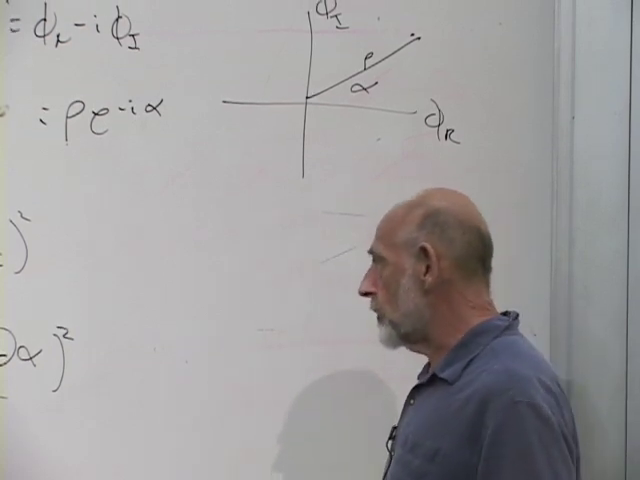
\includegraphics[width=0.72\textwidth]{lecture_08_figure_02.png}\caption{내부 \((\phi_R,\phi_I)\) 평면에 나타낸 복소 스칼라. 반지름은 \(\rho\)이고 \(\alpha\)는 내부 위상이다.}\lectureframe{00:24:41}\label{fig:l08-internal-plane}\end{figure}

스칼라 운동항은 다음과 같이 된다.
\begin{align}
  \partial_\mu\phi^*\,\partial^\mu\phi
  &=
  \partial_\mu\phi_R\,\partial^\mu\phi_R
  +\partial_\mu\phi_I\,\partial^\mu\phi_I
  \notag\\
  &=
  \partial_\mu\rho\,\partial^\mu\rho
  +\rho^2\partial_\mu\alpha\,\partial^\mu\alpha.
  \label{eq:l08-polar-kinetic}
\end{align}
전역적으로 \(U(1)\) 불변인 퍼텐셜은 \(\phi^*\phi=\rho^2\)에 의존하고 \(\alpha\)에는 의존하지 않는다. 예를 들면
\begin{equation}
  V(\phi)
  =\lambda\left(\phi^*\phi-\frac{f^2}{2}\right)^2,
  \qquad \lambda>0.
  \label{eq:l08-mexican-hat}
\end{equation}
최솟값들은 원을 이룬다. 물리 법칙은 공통 위상 회전에 대해 불변이지만, 평형 위상 하나를 택하면 그 원 위의 한 점이 선택된다.

\begin{figure}[htbp]\centering
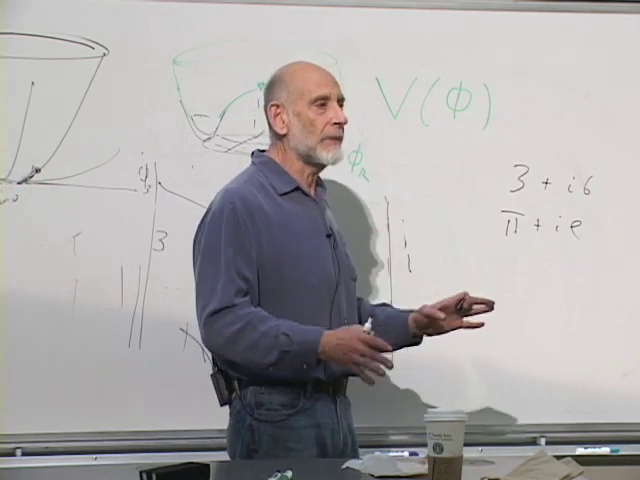
\includegraphics[width=0.78\textwidth]{lecture_08_figure_03.png}\caption{칠판에 그린 방사 방향 퍼텐셜 스케치. 장의 값이 원점에 있지 않더라도 퍼텐셜은 내부 장 값의 회전에 대해 대칭이다.}\lectureframe{00:34:22}\label{fig:l08-radial-potential-board}\end{figure}

\begin{figure}[htbp]\centering
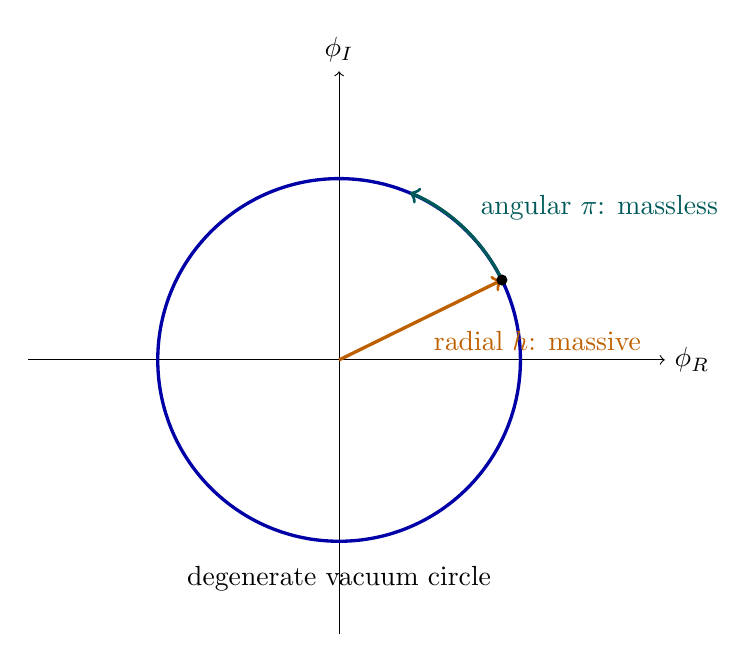
\begin{tikzpicture}[x=0.94cm,y=0.94cm]
  \draw[->] (-4.2,0) -- (4.4,0) node[right] {\(\phi_R\)};
  \draw[->] (0,-3.7) -- (0,3.9) node[above] {\(\phi_I\)};
  \draw[very thick,blue!65!black] (0,0) circle (2.45);
  \draw[->,very thick,orange!75!black] (0,0) -- (2.2,1.08);
  \draw[->,very thick,teal!70!black]
    (2.2,1.08) arc[start angle=26,end angle=67,radius=2.45];
  \node[orange!75!black,below right] at (1.15,0.52)
    {radial \(h\): massive};
  \node[teal!70!black,above right] at (1.78,1.76)
    {angular \(\pi\): massless};
  \fill (2.2,1.08) circle (2pt);
  \node[below] at (0,-2.65) {degenerate vacuum circle};
\end{tikzpicture}\caption{전역 대칭이 깨진 이론에서 진공 원에 수직인 방향으로는 곡률이 있지만, 원을 따라가는 방향으로는 곡률이 없다. 방사 방향 힉스 모드는 질량이 있고, 각방향 골드스톤 모드는 질량이 없다.}\label{fig:l08-radial-angular}\end{figure}

다음과 같이 두자.
\begin{equation}
  \phi(x)=\frac{f+h(x)}{\sqrt2}
           e^{i\pi(x)/f}.
  \label{eq:l08-canonical-polar}
\end{equation}
선택된 진공 근처에서 \(h\)는 방사 방향 변위를 나타내고, \(\pi\)는 정준 차원으로 접선 방향 변위를 나타낸다. 식~\eqref{eq:l08-polar-kinetic}에 대입하면
\begin{equation}
  \partial_\mu\phi^*\,\partial^\mu\phi
  =
  \frac12(\partial_\mu h)^2
  +\frac12\left(1+\frac{h}{f}\right)^2
            (\partial_\mu\pi)^2.
  \label{eq:l08-global-expanded}
\end{equation}
식~\eqref{eq:l08-mexican-hat}의 퍼텐셜은 다음을 준다.
\begin{equation}
  m_h^2=2\lambda f^2,
  \qquad
  m_\pi^2=0.
  \label{eq:l08-global-masses}
\end{equation}
\(m_h\)보다 훨씬 낮은 에너지에서는 방사 방향 운동에 큰 에너지가 들므로, 일시적으로 \(h=0\)으로 고정할 수 있다. 남는 라그랑지언에는 \(\frac12(\partial\pi)^2\)만 있고 \(\pi^2\) 항은 없다. 이것이 골드스톤 보손이다.\editorialnote{구두 설명에서는 두 지점에서 명칭을 뒤바꾸어 골드스톤을 흡수하면서 힉스 보손이 질량을 얻는다고 말한다. 그러나 칠판의 계산과 강의 나머지 내용은 의도된 결과를 보여 준다. 방사 방향 곡률이 이미 힉스 모드에 질량을 주며, 게이지 보손은 골드스톤 모드를 흡수하여 질량을 얻는다.}

\begin{classroomqa}\audiencequestion{표준모형에서 자발 대칭 깨짐은 이것뿐인가요?\lecturetimestamp{00:16:39}}\lecturerresponse{여기서 관련된 확립된 대칭 깨짐 메커니즘은 전약 힉스 상이다. 실제 대칭은 이 단일 \(U(1)\)가 아니라 \(SU(2)_L\times U(1)_Y\)이며, QCD 진공에도 카이랄 대칭 깨짐과 같은 추가 구조가 있다. 아벨 예제는 게이지 보손 메커니즘만을 의도적으로 축소해 보여 주는 모형이다.}\end{classroomqa}

\begin{classroomqa}
\audiencequestion{힉스장은 자기 자신을 포함한 모든 입자에 질량을 부여하는가?\lecturetimestamp{00:17:11}}
\lecturerresponse{그렇기도 하고 아니기도 하다. 전약 대칭성은 \(W\), \(Z\) 및 표준모형 페르미온의 맨질량을 금지한다. 이들의 질량은 힉스장이 영이 아닌 평형 크기를 갖게 된 뒤 생긴다. 방사 방향 힉스 질량은 힉스 퍼텐셜 자체의 곡률에서 비롯된다. 다른 가상 입자들은 이 메커니즘과 무관하게 대칭성이 허용하는 질량을 가질 수도 있다.}
\end{classroomqa}

강의에서는 대칭이 허용하는 이런 질량을 매우 무거워 관측하기 어려울 수 있는 입자와 연결하며, 암흑물질을 가능한 사례로 언급한다. 이는 동기를 제시하는 말이지 질량을 예측하는 말은 아니다.
\editorialnote{암흑물질의 질량 척도는 아직 알려져 있지 않다. 강의에서 양성자 질량의 약 천 배인 입자를 제안한 것은 역사적 추측이지, 실험으로 확립된 암흑물질의 성질이 아니다.}

\begin{classroomqa}\audiencequestion{\(\rho\)는 물리적 반지름인가요, 아니면 장의 값인가요? 무엇이 정확히 방사 대칭인가요?\lecturetimestamp{00:33:08}}\lecturerresponse{각 시공간 점에서 장의 값은 보조 복소 평면의 한 점이고, \(\rho=|\phi|\)는 그 점에서 원점까지의 거리다. \emph{퍼텐셜}은 이 내부 평면에서 방사 대칭이다. 즉 같은 \(\rho\)를 가진 모든 점은 퍼텐셜 에너지가 같다. 이 반지름은 보통 공간에서의 거리가 아니다.}\end{classroomqa}

\begin{classroomqa}\audiencequestion{방사 방향으로 충분히 세게 밀면 장이 중앙의 최대점을 넘어 퍼텐셜의 반대편으로 갈 수 있나요?\lecturetimestamp{00:36:00}}\lecturerresponse{원리상 충분한 에너지가 있는 국소 배치는 장벽을 넘어갈 수 있다. 균일한 거시적 장을 장벽 너머로 옮기려면 막대한 에너지가 필요하며, 일반적인 격렬한 교란은 반대편 점에 결맞게 도달하기보다 여러 장 모드로 에너지를 방출한다. 저에너지 근사에서 \(\rho\)를 고정하는 이유는 바로 그런 방사 방향 이탈이 그 범위에서는 일어나기 어렵기 때문이다.}\end{classroomqa}

\section{복소 평면은 왜 시공간이 아닌가}

물리 좌표와 내부 좌표의 구분은 강의에서 충분히 짚고 넘어갈 만하다. 스칼라장이 스칼라라고 불리는 이유는 물리적 좌표축의 회전 아래 불변이기 때문이다. 두 실수 스칼라장 \(\phi_R(x)\)와 \(\phi_I(x)\)는 그런 회전 아래에서도 각각 스칼라로 남는다. 둘을 하나의 복소수로 묶을 수는 있지만, 이는 표기상의 편의일 뿐 이들을 공간 벡터의 성분으로 바꾸지 않는다.

전역 \(U(1)\) 변환은 장의 \emph{값}을 회전시킨다.
\begin{equation}
\begin{aligned}
  \phi(x)&\longmapsto e^{i\theta}\phi(x),
  \\
  \rho(x)&\longmapsto\rho(x),
  \\
  \alpha(x)&\longmapsto\alpha(x)+\theta.
\end{aligned}
  \label{eq:l08-global-shift}
\end{equation}
모든 시공간 점에서 같은 상수 \(\theta\)를 사용한다. 따라서 \(\partial_\mu\alpha\)는 변하지 않는다. 이는 퍼텐셜과 일반적인 운동항 모두의 대칭이다. \(\theta\)가 \(x\)에 따라 달라지도록 허용하면 미분이 그 변화를 감지하므로 논의가 달라진다.

\section{위상 회전을 국소적으로 만들기}

\subsection{일반 미분의 실패}

다음과 같이 두자.
\begin{equation}
  \phi'(x)=e^{i\theta(x)}\phi(x).
  \label{eq:l08-local-phase}
\end{equation}
그러면
\begin{equation}
  \partial_\mu\phi'
  =e^{i\theta}
    \left(\partial_\mu\phi+i\,\partial_\mu\theta\,\phi\right).
  \label{eq:l08-ordinary-derivative-fails}
\end{equation}
\(\partial_\mu\theta\)에 비례하는 추가 항 때문에 \(\partial_\mu\phi\)는 \(\phi\)처럼 변환하지 않는다. 따라서 임의의 국소 위상 회전 아래에서는 \(\partial_\mu\phi^*\partial^\mu\phi\)가 불변이 아니다.

\begin{figure}[htbp]\centering
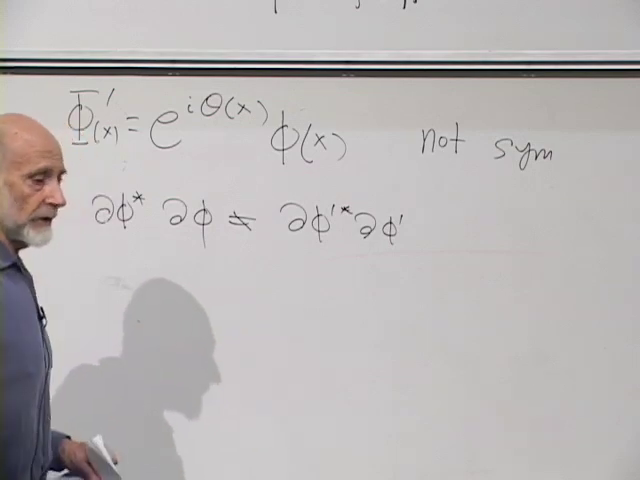
\includegraphics[width=0.78\textwidth]{lecture_08_figure_04.png}\caption{칠판에는 국소 위상 변환과 일반 미분 항이 불변성을 유지하지 못하는 과정이 적혀 있다.}\lectureframe{00:46:49}\label{fig:l08-local-not-symmetry}\end{figure}

벡터 퍼텐셜을 도입하고 하나의 규약을 일관되게 정하자.
\begin{equation}
  D_\mu=\partial_\mu+i g A_\mu,
  \qquad
  A_\mu'=A_\mu-\frac1g\partial_\mu\theta.
  \label{eq:l08-covariant-convention}
\end{equation}
이제
\begin{align}
  D_\mu'\phi'
  &=
  \left(\partial_\mu+i g A_\mu'\right)
  e^{i\theta}\phi
  \notag\\
  &=
  e^{i\theta}
  \left[
    \partial_\mu\phi+i(\partial_\mu\theta)\phi
    +i g A_\mu\phi-i(\partial_\mu\theta)\phi
  \right]
  \notag\\
  &=e^{i\theta}D_\mu\phi.
  \label{eq:l08-covariant-transform}
\end{align}
원치 않는 항들이 상쇄된다. 켤레 미분은
\begin{equation}
  (D_\mu\phi)^*
  =(\partial_\mu-i g A_\mu)\phi^*,
\end{equation}
이며, 그 반대 위상은 곱에서 상쇄된다.
\begin{equation}
  (D_\mu\phi)^*D^\mu\phi.
\end{equation}

\begin{classroomqa}\audiencequestion{지난 강의에서는 게이지장 변환을 반대 부호로 썼나요?\lecturetimestamp{00:48:04}}\lecturerresponse{\(D_\mu\)의 부호와 변환 법칙의 부호를 함께 뒤집는 것은 단지 규약의 차이다. \(D_\mu=\partial_\mu+i gA_\mu\)와 \(\phi'=e^{i\theta}\phi\)를 쓰면 일관성을 위해 \(A_\mu'=A_\mu-g^{-1}\partial_\mu\theta\)이어야 한다. 모든 부호를 함께 바꾸면 다른 규약도 똑같이 잘 작동한다.}\end{classroomqa}

\begin{classroomqa}\audiencequestion{칠판에 \(\phi\)를 대문자 또는 소문자 형태로 쓴 것은 서로 다른 장을 뜻하나요?\lecturetimestamp{00:55:02}}\lecturerresponse{그런 구분은 의도된 것이 아니다. 글자 모양이 바뀐 것은 손글씨 때문이지, 별도의 연산이나 두 번째 스칼라가 있어서가 아니다. 의미 있는 구분은 프라임, 복소켤레 별표, 시공간 지수다.}\end{classroomqa}

\begin{classroomqa}\audiencequestion{운동항에서 복소켤레를 취하는 것은 로런츠 지수를 올리거나 내리는 것과 같은 연산인가요?\lecturetimestamp{00:56:50}}\lecturerresponse{아니다. 별표는 내부 복소장을 켤레화한다. 로런츠 지수는 시공간 계량으로 올린다.
\(D^\mu=g^{\mu\nu}D_\nu\). 로런츠 스칼라를 만들려면 \((D_\mu\phi)^*D^\mu\phi\)와 같이 수축해야 한다. 두 연산은 모두 필요하지만 서로 다른 역할을 한다.}\end{classroomqa}

\subsection{게이지장에는 자체 동역학이 있다}

장세기
\begin{equation}
  F_{\mu\nu}=\partial_\mu A_\nu-\partial_\nu A_\mu
  \label{eq:l08-field-strength}
\end{equation}
는 \(\theta\)의 두 혼합 2계 미분이 서로 상쇄되므로 게이지 불변이다. 시간--공간 성분에는 전기장이, 공간--공간 성분에는 자기장이 들어 있다. 따라서 스칼라 전기역학의 라그랑지언은 다음과 같다.
\begin{equation}
  \mathcal L
  =(D_\mu\phi)^*D^\mu\phi
  -V(\phi^*\phi)
  -\frac14F_{\mu\nu}F^{\mu\nu}.
  \label{eq:l08-abelian-higgs}
\end{equation}
여기서 전하를 띤 장은 보손이다. 페르미온인 전자장은 아니다. 전하를 띤 헬륨 원자핵이나 쿠퍼쌍 응축은 전하를 띤 보손 자유도가 어떻게 생기는지 보여 주는 사례다.

대칭 깨짐 이전에 게이지 항에는 \(A_\mu\)의 미분은 들어 있지만 직접적인 질량 항은 없다. 다음 항을 더하려고 할 수 있다.
\begin{equation}
  \frac12m_A^2A_\mu A^\mu,
\end{equation}
하지만 식~\eqref{eq:l08-covariant-convention} 아래에서
\begin{equation}
  A_\mu A^\mu
  \longmapsto
  \left(A_\mu-\frac1g\partial_\mu\theta\right)
  \left(A^\mu-\frac1g\partial^\mu\theta\right),
  \label{eq:l08-bare-mass-fails}
\end{equation}
가 되어 \(A_\mu A^\mu\)와 같지 않다. 맨 게이지 보손 질량은 국소 대칭에 의해 금지된다.

\begin{figure}[htbp]\centering
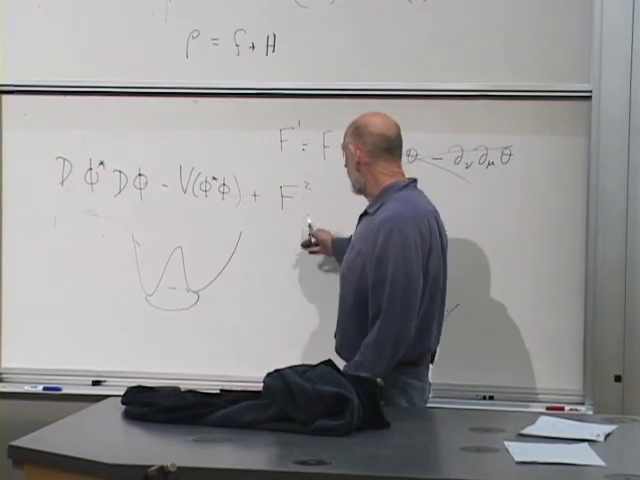
\includegraphics[width=0.76\textwidth]{lecture_08_figure_05.png}\caption{장애를 보여 주는 검증된 칠판 내용: 게이지 변환 아래에서 \(A_\mu A^\mu\)는 \(\partial_\mu\theta\)를 포함하는 제곱식으로 바뀌므로 맨 벡터 질량 항은 불변이 아니다.}\lectureframe{01:07:30}\label{fig:l08-bare-mass-board}\end{figure}

\section{힉스 메커니즘}

\subsection{공변 미분이 질량을 만든다}

깨진 퍼텐셜로 돌아가 정규화가 표준인 매개화를 사용하자.
\begin{equation}
  \phi(x)=\frac{f+h(x)}{\sqrt2}
  e^{i\pi(x)/f}.
\end{equation}
공변 미분은
\begin{equation}
  D_\mu\phi
  =
  \frac{e^{i\pi/f}}{\sqrt2}
  \left[
    \partial_\mu h
    +i(f+h)
      \left(\frac{\partial_\mu\pi}{f}+gA_\mu\right)
  \right].
  \label{eq:l08-covariant-polar}
\end{equation}
이므로
\begin{equation}
\begin{aligned}
  (D_\mu\phi)^*D^\mu\phi
  ={}&
  \frac12(\partial_\mu h)^2
  \\
  &+\frac12(f+h)^2
    \left(\frac{\partial_\mu\pi}{f}+gA_\mu\right)
  \\
  &\hspace{4.2em}\times
    \left(\frac{\partial^\mu\pi}{f}+gA^\mu\right).
\end{aligned}
  \label{eq:l08-higgs-kinetic}
\end{equation}

결정적인 항은 어떤 게이지를 선택하기도 전에 나타난다.
\begin{equation}
  \frac12g^2f^2 A_\mu A^\mu.
  \label{eq:l08-vector-mass-term}
\end{equation}
이를 프로카 형식 \(\frac12m_A^2A_\mu A^\mu\)과 비교하면 다음을 얻는다.
\begin{equation}
  \boxed{m_A=g f}.
  \label{eq:l08-vector-mass}
\end{equation}
같은 전개에서 상호작용 항 \(g^2fh A_\mu A^\mu\)과 \(\frac12g^2h^2A_\mu A^\mu\)도 생긴다. 따라서 벡터 질량은 게이지 대칭성을 임의로 깨뜨려 도입한 것이 아니다. 평형 크기 \(f\)가 영이 아닌 상에서 게이지 불변 스칼라 운동에너지 항을 계산하면 이 질량이 생긴다.

\begin{figure}[htbp]\centering
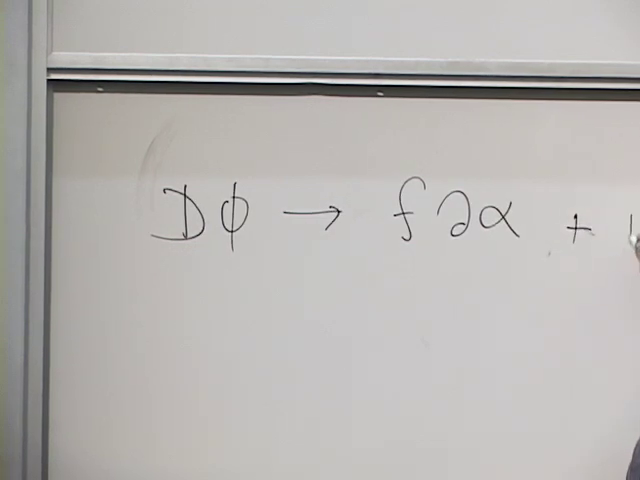
\includegraphics[width=0.78\textwidth]{lecture_08_figure_06.png}\caption{칠판에서 \((D\phi)^*(D\phi)\) 안의 \(f^2A^2\) 기여 항을 따로 뽑아 보인다. 수치 계수는 스칼라장과 게이지 결합을 어떻게 정규화하느냐에 따라 달라진다. 식~\eqref{eq:l08-canonical-polar}와 \eqref{eq:l08-covariant-convention}를 사용하면 결과는 \(m_A=gf\)이다.}\lectureframe{01:10:10}\label{fig:l08-generated-mass-board}\end{figure}

강의에서는 \(g\)와 \(\sqrt2\)의 여러 계수를 칠판 표기 안에 흡수하므로, 질량을 식별하는 대목에서 \(f\), \(2f\), \(\sqrt2f\)를 번갈아 사용한다. 운동항과 퍼텐셜의 정규화를 밝히기 전에는 이 계수들에 불변적인 의미가 없다. 견고한 결과는 \(m_A\propto gf\)이며, 식~\eqref{eq:l08-vector-mass}은 여기서 사용한 규약에 따른 계수를 준다.

\subsection{위상을 흡수하기}

게이지 변환 아래에서 위상 변수는 다음과 같이 변한다.
\begin{equation}
  \pi'(x)=\pi(x)+f\,\theta(x).
\end{equation}
다음과 같이 택하자.
\begin{equation}
  \theta(x)=-\frac{\pi(x)}{f}.
  \label{eq:l08-unitary-gauge-choice}
\end{equation}
그러면 \(\pi'=0\)이다. 이것이 유니터리 게이지이며, 이 게이지에서는 \begin{equation}
  \phi'(x)=\frac{f+h(x)}{\sqrt2}
\end{equation}가 실수다. 식~\eqref{eq:l08-higgs-kinetic}은 다음과 같이 단순해진다.
\begin{equation}
  (D_\mu\phi')^*D^\mu\phi'
  =
  \frac12(\partial_\mu h)^2
  +\frac12g^2(f+h)^2A_\mu'A^{\prime\mu}.
  \label{eq:l08-unitary-gauge-lagrangian}
\end{equation}
각방향 골드스톤 장은 독립 변수 목록에서 사라지지만, 벡터 질량은 남는다.

강의에서는 먼저 저에너지 극한 \(\rho=f\)에서 이를 보인다. 이때
\begin{align}
  \phi&=f e^{i\alpha},
  \notag\\
  D_\mu\phi
  &=if e^{i\alpha}
    \left(\partial_\mu\alpha+gA_\mu\right),
  \notag\\
  (D_\mu\phi)^*
  &=-if e^{-i\alpha}
    \left(\partial_\mu\alpha+gA_\mu\right).
  \label{eq:l08-frozen-radius}
\end{align}
두 식의 곱은
\begin{equation}
  f^2
  \left(\partial_\mu\alpha+gA_\mu\right)
  \left(\partial^\mu\alpha+gA^\mu\right).
\end{equation}
이다. \(\theta=-\alpha\)를 택하면 \(g^2f^2A_\mu'A^{\prime\mu}\)가 남는다.

\begin{figure}[htbp]\centering
\includegraphics[width=0.82\textwidth]{lecture_08_figure_07.png}\caption{반지름을 고정한 완전한 칠판 전개: 공변 미분에는 위상 미분과 벡터 퍼텐셜이 함께 들어 있다. 이어서 강의에서는 \(\theta=-\alpha\)를 택해 위상을 없애고 벡터 질량 항을 남긴다.}\lectureframe{01:16:20}\label{fig:l08-frozen-radius-board}\end{figure}

\begin{classroomqa}\audiencequestion{각방향 모드가 사라지는 것을 명시적으로 보여 주는 변수로 라그랑지언 전체를 다시 쓸 수 있나요?\lecturetimestamp{01:13:49}}\lecturerresponse{그렇다. 극좌표 변수에서는 위상이 게이지 불변 조합 \(\partial_\mu\alpha+gA_\mu\)에만 나타난다. 이 게이지가 잘 정의되는 모든 곳에서 \(\theta=-\alpha\)인 게이지 변환을 택하면 위상을 0으로 만들 수 있다. 그러면 스칼라 운동항은 벡터 질량 항이 되고, 게이지 불변 장세기 항은 변하지 않는다.}\end{classroomqa}

\begin{classroomqa}\audiencequestion{\(\alpha\)의 진동은 게이지장의 진동과 구별할 수 없나요?\lecturetimestamp{01:18:02}}\lecturerresponse{게이지 이론에서 이에 대응하는 \(A_\mu\)의 변화로 상쇄되는 \(\alpha\)의 순수한 변화는 서로 다른 물리적 파동이 아니라 게이지에 따른 재기술이다. 불변량은 \(\partial_\mu\alpha+gA_\mu\)다. 전역 골드스톤 장으로 표현되던 물리적 모드는 질량 있는 벡터의 종방향 편광으로 다시 나타난다.}\end{classroomqa}

국소 게이지 대칭성이 자발적으로 깨진다고 흔히 말한다. 게이지를 선택한 뒤 스칼라장이 영이 아닌 진공값을 갖고 스펙트럼에 질량이 있는 벡터가 포함된다는 점에서 이 표현은 실용적으로 유용하다. 그러나 엄밀히 말해 게이지 변환은 서로 다른 물리적 상태가 아니라 중복된 기술들을 서로 대응시킨다.
\editorialnote{국소 게이지 중복성은 전역 대칭성과 같은 게이지 불변적 의미에서 깨지는 것이 아니다. 정확히 말하면 이론은 힉스 상에 있다. 게이지 고정 섭동 이론에서는 이 상을 영이 아닌 스칼라 기댓값과 그에 따른 질량 있는 벡터 스펙트럼으로 기술한다.}

\section{골드스톤 자유도는 어디로 갔는가}

변수를 바꾸었다고 해서 물리적인 것이 사라질 수는 없다. 힉스 상에 들어가기 전후의 자유도를 세어 보자.

그 전에는
\begin{equation}
  \underbrace{2}_{\text{massless vector}}
  +
  \underbrace{2}_{\text{complex scalar}}
  =4.
\end{equation}
질량 없는 벡터에는 횡편광이 두 개 있다. 복소 스칼라에는 방사 방향과 각방향의 두 실수 성분이 있다.

그 뒤에는
\begin{equation}
  \underbrace{3}_{\text{massive vector}}
  +
  \underbrace{1}_{\text{radial Higgs}}
  =4.
  \label{eq:l08-degree-count}
\end{equation}
질량 있는 벡터는 정지 상태로 만들 수 있다. 정지계에서는 특별히 선택되는 공간 방향이 없으므로 편광 상태가 세 개여야 한다. 벡터가 움직일 때 그중 둘은 횡방향이고 하나는 종방향이다. 골드스톤 모드는 이 종방향 편광이 되었다.

\begin{figure}[htbp]\centering
\begin{adjustbox}{max width=\linewidth}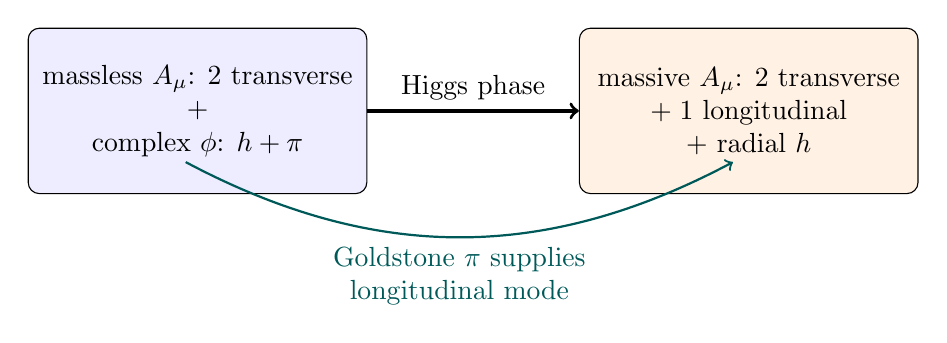
\begin{tikzpicture}[x=1cm,y=1cm]
  \node[draw,rounded corners,fill=blue!7,minimum width=4.3cm,
        minimum height=2.1cm,align=center] (before) at (0,0)
    {massless \(A_\mu\): \(2\) transverse\\
     \(+\)\\
     complex \(\phi\): \(h+\pi\)};
  \node[draw,rounded corners,fill=orange!10,minimum width=4.3cm,
        minimum height=2.1cm,align=center] (after) at (7,0)
    {massive \(A_\mu\): \(2\) transverse\\
     \(+\;1\) longitudinal\\
     \(+\) radial \(h\)};
  \draw[->,very thick] (before) -- node[above]{Higgs phase} (after);
  \draw[->,teal!70!black,thick]
    (-0.15,-0.65) to[bend right=28]
    node[below,align=center]{Goldstone \(\pi\) supplies\\longitudinal mode}
    (6.8,-0.65);
\end{tikzpicture}\end{adjustbox}\caption{힉스 메커니즘은 물리적 자유도를 없애는 것이 아니라 재배열한다.}\label{fig:l08-degree-rearrangement}\end{figure}

\begin{classroomqa}\audiencequestion{자유도 수를 어기지 않으면서 각방향 자유도가 어떻게 사라질 수 있나요?\lecturetimestamp{01:19:13}}\lecturerresponse{물리적으로 사라지는 것은 아니다. 질량 없는 벡터는 정지 상태로 만들 수 없기 때문에 헬리시티가 두 개다. 질량 있는 벡터에는 종방향을 포함해 편광 상태가 세 개 있다. 골드스톤 모드가 세 번째 편광이 되므로 전체 자유도 수는 그대로다.}\end{classroomqa}

강의에서는 유용한 운동학적 검증 방법을 제시한다. 질량이 있는 벡터 입자를 생각해 정지 상태까지 감속한 다음 새로운 방향으로 가속한다고 하자. 원래 운동 방향에 대해 횡방향이던 편광이 새로운 운동 방향에 대해서는 종방향이 될 수 있다. 마찬가지로 원편광된 질량 있는 입자를 정지 상태로 옮겼다가 반대 방향으로 보내면 헬리시티 표지가 뒤집힌다. 엄밀히 질량이 없는 입자는 어떤 관성계에서도 정지 상태가 될 수 없으므로 이 실험을 거칠 수 없다. 따라서 그 두 헬리시티는 일관된 물리적 스펙트럼을 이룬다.

\section{초전도체와의 유사성}

일반적인 초전도체에서는 전자들이 쿠퍼 쌍을 이룬다. 쿠퍼 쌍은 전하 \(2e\)를 띤 보손이며, 응축체는 전하를 띤 복소 질서 매개변수로 기술된다. 그 크기가 영이 아니면 질서 매개변수의 위상과 전자기 벡터 퍼텐셜의 결합으로 앤더슨--힉스 메커니즘이 나타난다. 정적 자기장은 런던 침투 깊이를 따라 감쇠하므로 초전도체 내부로 자유롭게 뻗어 나가지 않는다. 이처럼 특정 매질에 한정된 정확한 의미에서 광자는 질량을 얻은 것처럼 거동한다.

이 사례는 처음에 제시한 구분도 명확히 해 준다. 전자기장이 영구적으로 다른 기본 입자로 바뀌는 것은 아니다. 질량 있는 전파 법칙은 물질 내부의 집단 상태에 해당하며, 바깥의 진공 광자는 여전히 질량이 없다.

\section{확립된 결과}

논리를 유지하면서 이제 논증을 간결하게 정리할 수 있다.
\begin{enumerate}
  \item 깨진 전역 연속 대칭성에는 평평한 각방향이 있으므로 질량이 없는 골드스톤 모드가 존재한다.
  \item 국소 위상 불변성은 게이지 퍼텐셜을 요구하며 \(\partial_\mu\)를 \(D_\mu\)로 대체한다.
  \item 맨 \(A_\mu A^\mu\) 질량은 국소 변환 법칙을 위반한다.
  \item 전하를 띤 스칼라의 평형 크기 \(f\)가 영이 아니면 게이지 불변 항 \(|D_\mu\phi|^2\)에 \(\frac12g^2f^2A_\mu A^\mu\)가 포함된다.
  \item 게이지를 선택하면 위상을 제거할 수 있으며, 그 물리적 자유도는 질량이 있는 벡터의 종방향 편극이 된다.
  \item 방사 방향 힉스 여기자의 질량은 스칼라 퍼텐셜의 곡률로 정해진다.
\end{enumerate}

다음 과제는 페르미온에 질량을 부여하는 것이다. 전자와 쿼크에는 벡터 메커니즘을 직접 적용할 수 없다. 이들의 힉스 결합은 유카와 상호작용이다. 스칼라장이 \(f\)에 자리 잡으면 이 상호작용은 페르미온 질량 항이 된다.

전약 대칭성 깨짐이 없으면 익숙한 입자들이 질량이 없었을 것이라는 폭넓은 진술에는 마지막으로 단서를 붙여야 한다. 기본 입자인 쿼크와 하전 렙톤의 질량, 그리고 \(W\) 및 \(Z\)의 질량은 힉스 기댓값이 영이 되면 사라진다. 그러나 양성자와 중성자 질량의 대부분은 쿼크의 힉스 질량이 아니라 QCD 가둠과 강한 장의 에너지에서 동역학적으로 비롯된다. 이 구분은 여기서 유도한 힉스 메커니즘을 바꾸지 않으며, 그 적용 범위를 정확히 한정해 준다.
